\begin{frame}[allowframebreaks]{Clustering - Hierarchical}
\begin{columns}
    \begin{column}{0.45\textwidth}
        Cluster based on distances  between observations.

        \vspace{0.8em}

        Represented as a tree hierarchy  (\textit{dendrogram}) rather than a  partition of data.

        \vspace{0.8em}

        Does not require committing to a  choice of $K$.
    \end{column}
    \begin{column}{0.55\textwidth}
        \begin{figure}
            \centering
            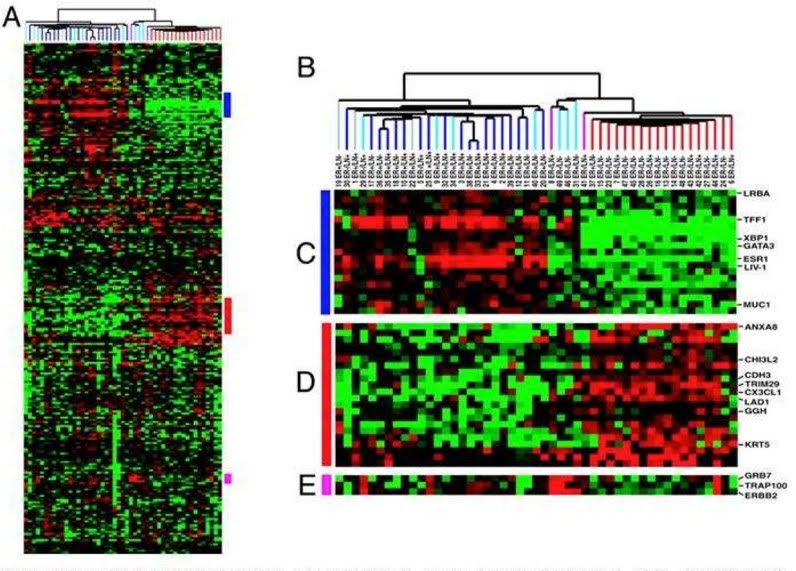
\includegraphics[width=0.8\textwidth,keepaspectratio]{images/dul/hierarchical/breast-tumor-subtypes.jpg}
            \caption{Sørlie, Therese, et al. (2003) "Repeated observation of breast  tumor subtypes in independent gene expression data sets," PNAS.}
        \end{figure}
    \end{column}
\end{columns}
\end{frame}

\begin{frame}[allowframebreaks]{Clustering - Hierarchical: Dendrograms}
\begin{columns}
    \begin{column}{0.45\textwidth}
        \begin{itemize}
            \setlength{\itemsep}{0.5em}
            \item Each leaf in a dendrogram is a sample/  observation.
            \item As we move up the dendrogram, observations  that are similar to each other begin to fuse  into branches.
            \item Branches then fuse into bigger branches.
            \item Observations that fuse later (near the top of  the tree, or root) are more different than observations that fuse earlier (near the leaves).
        \end{itemize}
    \end{column}

    \vspace{0.8em}

    \begin{column}{0.55\textwidth}
        \begin{figure}
            \centering
            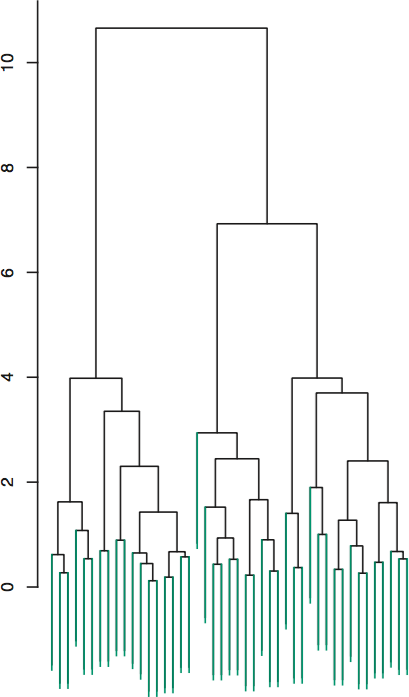
\includegraphics[width=0.95\textwidth,height=0.8\textheight,keepaspectratio]{images/dul/hierarchical/dendrograms.png}
            \caption{ISL (8th printing 2017)}
        \end{figure}
    \end{column}
\end{columns}

\framebreak

\begin{block}{}
    Note that the horizontal distance between observations on a  dendrogram is not the appropriate assessment of observation  similarity. Instead, look at vertical axis where branches are first fused.

    \vspace{1.5em}

    \begin{figure}
        \centering
        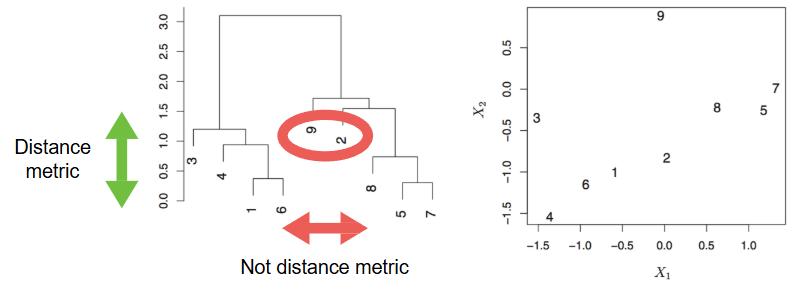
\includegraphics[width=0.95\textwidth,height=0.7\textheight,keepaspectratio]{images/dul/hierarchical/dendograms-distance-metric.png}
        \caption{ISL (8th printing 2017)}
    \end{figure}
\end{block}

\framebreak

\begin{columns}
    \begin{column}{0.45\textwidth}
        Clusters are created by  making a horizontal cut  across the dendrogram.  Clusters are the separate  trees below the cut.
    \end{column}

    \vspace{0.8em}

    \begin{column}{0.55\textwidth}
        \begin{figure}
            \centering
            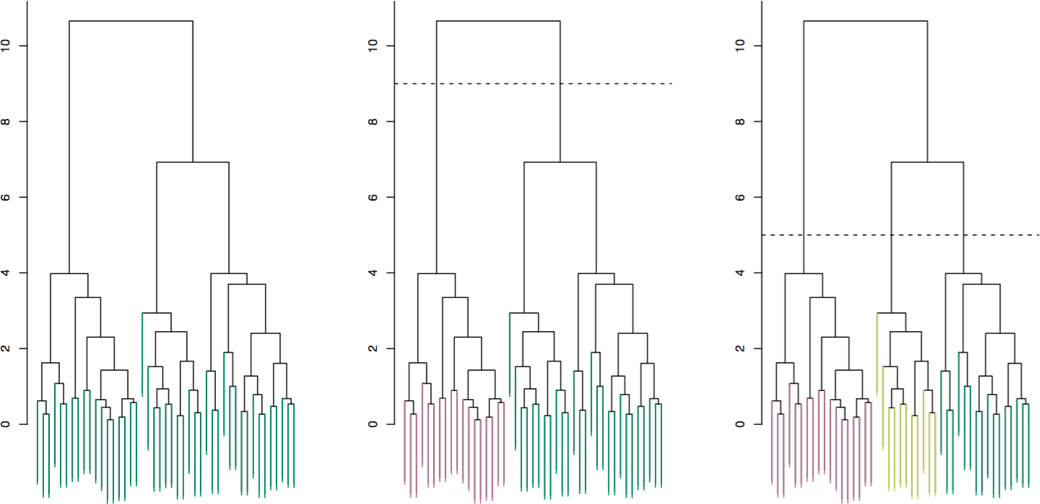
\includegraphics[width=1.05\textwidth,height=0.8\textheight,keepaspectratio]{images/dul/hierarchical/dendrograms-cluster.png}
            \caption{ISL (8th printing 2017)}
        \end{figure}
    \end{column}
\end{columns}

\framebreak

\begin{block}{Building a Dendrogram}
    A dendrogram is most commonly built using a bottom-up or agglomerative algorithm.

    \vspace{0.8em}

    We start at the leaves and group observations until we reach the root  containing the entire dataset.
    
    \vspace{0.8em}

    Like in $k$-means, we need a measure of similarity. Again, the most  common is Euclidean distance.

    \vspace{0.8em}

    \begin{itemize}
        \setlength{\itemsep}{0.5em}
        \item Compute the distance between each pair of observations.
        \item Merge the two closest observations into a cluster.
        \item Compute the distance between the new cluster and all other observations.
        \item Repeat until all observations are in one cluster.
        \item The distance between clusters is computed using a linkage method.
    \end{itemize}
\end{block}

\framebreak

% Hierarchical clustering Algorithm - pseudo code
\begin{algorithm}[H]
\caption{Hierarchical Clustering Algorithm}
\KwIn{Dataset $D = \{x_1, x_2, \dots, x_n\}$}
\KwOut{Dendrogram representing the hierarchical structure of clusters}
\textbf{Initialization:} Treat each data point as a separate cluster\;
\textbf{Compute distance matrix:} Calculate pairwise distances between all clusters\;
\textbf{Repeat until only one cluster remains:}
\begin{itemize}
    \item Find the two closest clusters based on the distance matrix\;
    \item Merge the two clusters into a new cluster\;
    \item Update the distance matrix to reflect the new cluster\;
    \item Recompute distances between the new cluster and all other clusters using a linkage method\;
\end{itemize}
\textbf{Return:} Dendrogram representing the hierarchical structure of clusters\;
\end{algorithm}

\href{https://www.w3schools.com/python/python_ml_hierarchial_clustering.asp}{w3schools: Codes and Playground}

\framebreak

\begin{figure}
    \centering
    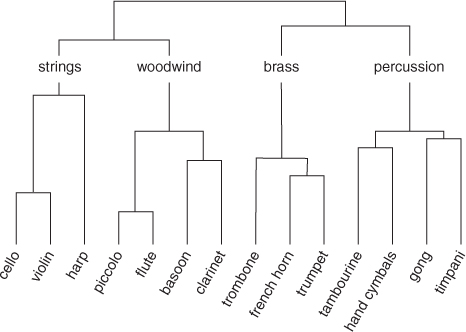
\includegraphics[width=0.95\textwidth,height=0.85\textheight,keepaspectratio]{images/dul/hierarchical/dendrogram-interpretation.png}
    \caption{Dendrogram interpretation.}
\end{figure}
\end{frame}


\begin{frame}[allowframebreaks]{Clustering - Hierarchical: Distance Metrics}
\vspace*{-2em}
\begin{block}{Distance between groups}
    It’s easy to compute Euclidean distance between two observations.  What is the distance or similarity between two groups or clusters of  observations?
    
    \vspace{0.8em}
    \textbf{Linkage}: defines the dissimilarity between two groups of observations.  Most common types are $complete$, $average$, $single$, and $centroid$.
\end{block}

\framebreak

\begin{itemize}
    \setlength{\itemsep}{0.5em}
    \item \textbf{Single Linkage}: Distance between two clusters is the minimum distance between any two points in the clusters.
    \item \textbf{Complete Linkage}: Distance between two clusters is the maximum distance between any two points in the clusters.
    \item \textbf{Average Linkage}: Distance between two clusters is the average distance between all pairs of points in the clusters.
    \item \textbf{Centroid Linkage}: Distance between two clusters is the distance between their centroids.
    \item \textbf{Ward's Linkage}: Distance between two clusters is the increase in variance when the two clusters are merged.
\end{itemize}

\framebreak

\begin{figure}
    \centering
    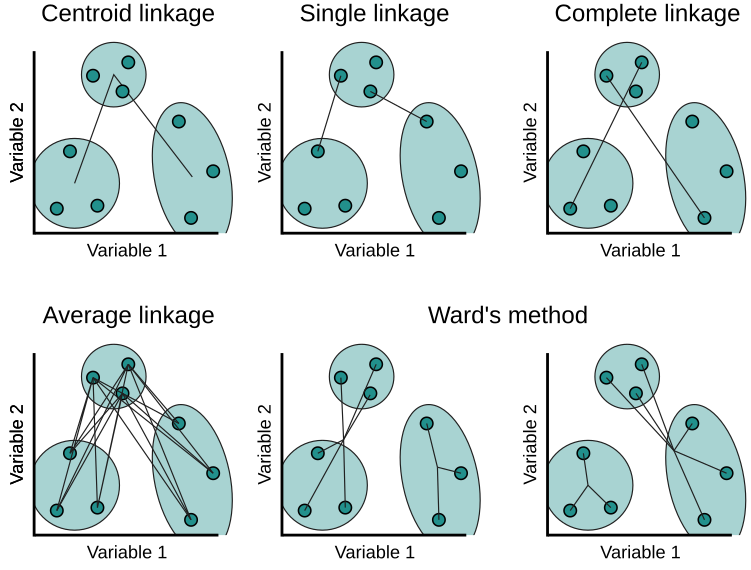
\includegraphics[width=0.95\textwidth,height=0.85\textheight,keepaspectratio]{images/dul/hierarchical/linkage.png}
    \caption{Linkage methods.}
\end{figure}

\begin{figure}
    \centering
    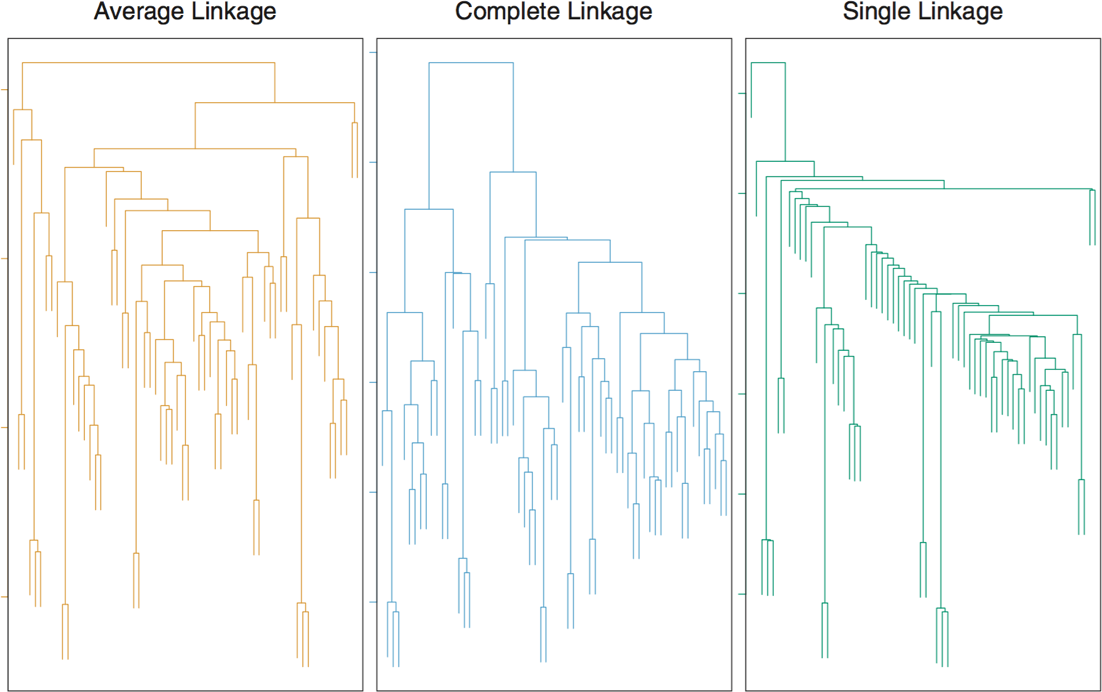
\includegraphics[width=0.95\textwidth,height=0.85\textheight,keepaspectratio]{images/dul/hierarchical/dendrogram-linkage-types.png}
    \caption{Dendrogram with different linkage types.}
\end{figure}
\end{frame}


\begin{frame}[allowframebreaks]{Clustering - Hierarchical: Pros and Cons}
\begin{columns}
    \begin{column}{0.5\textwidth}
        \textbf{Pros}
        \begin{itemize}
            \setlength{\itemsep}{1em}
            \item No need to specify the number of clusters $K$ in advance.
            \item Dendrograms provide a visual representation of the clustering process.
            \item Can capture complex cluster shapes and relationships.
        \end{itemize}
    \end{column}
    \begin{column}{0.5\textwidth}
        \textbf{Cons}
        \begin{itemize}
            \setlength{\itemsep}{1em}
            \item Computationally expensive for large datasets.
            \item Do have to pick where to cut the dendrogram to obtain clusters
            \item Sensitive to similarity measure and type of linkage used.
            \item Sensitive to noise and outliers.
            \item Difficult to interpret and choose the optimal number of clusters.
        \end{itemize}
    \end{column}
\end{columns}
\end{frame}
